\section{Using AccLab web UI}
To run the web ui :

{
\lstset{style=shell}
\begin{lstlisting}
root@root/:$ python aalc.py -u 8000
\end{lstlisting}
}


\begin{figure}[!ht]
      \center
      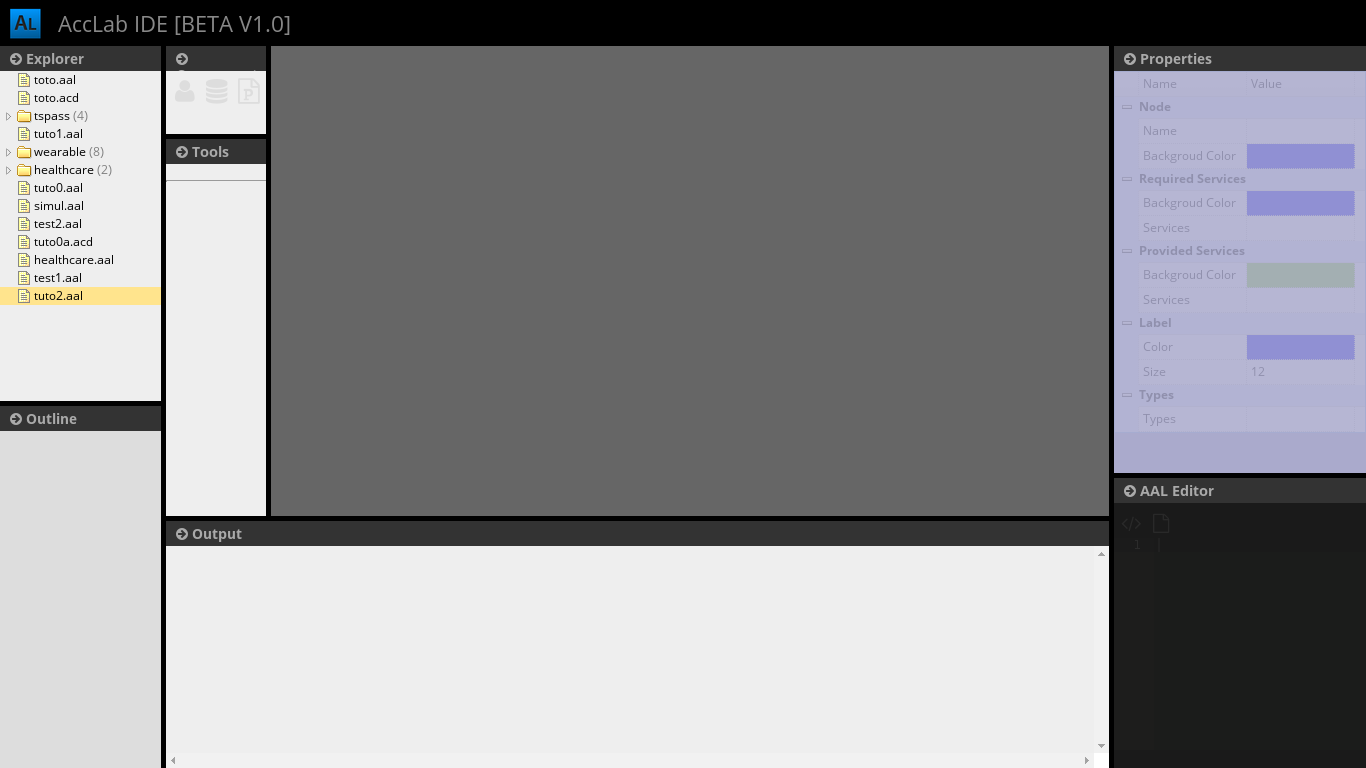
\includegraphics[width=15cm,angle=0]{assets/gui/interface0.png}
      \caption{ACD Editor}
\end{figure}

\begin{enumerate}
    \item \textbf{Explorer :} This panel contains a tree view of the your workspace (-\texttt{*.aal} a
    simple text format that contains AAL code; -\texttt{*.acd} a json file format that contains the components diagram)
    \item \textbf{Outline :} The outline contains a tree view of the current components (with blue icon) in the
    opened \texttt{acd} file, and for each agent its required services (in red icon) and provided services (green icon).
    \item \textbf{Components :} Contains the elements that can be used in the diagram (\texttt{agent :} a simple agent
     with types, required and provided services; \texttt{data :} same as agent but with an additional attribute \texttt{subject} (the data owner) ; macro : insert a macro call in the generated AAL program (more details will be provided soon)).
    \item \textbf{Tools :} A panel containing different tools to be used while editing acd/aal files (copy/past/zoom/save/etc).
    \item \textbf{Diagram :} The diagram.
    \item \textbf{Properties :} A grid containing the properties of a selected element in the diagram, in which you
    can edit its name, style properties (color, font, etc) and also types/services.
    \item \textbf{Output :} The output where we show the result coming from the back-end.
    \item \textbf{AAL editor :} Allows to edit quickly a component's policy, before generating the AAL program.
\end{enumerate}


\begin{figure}[!ht]
      \center
      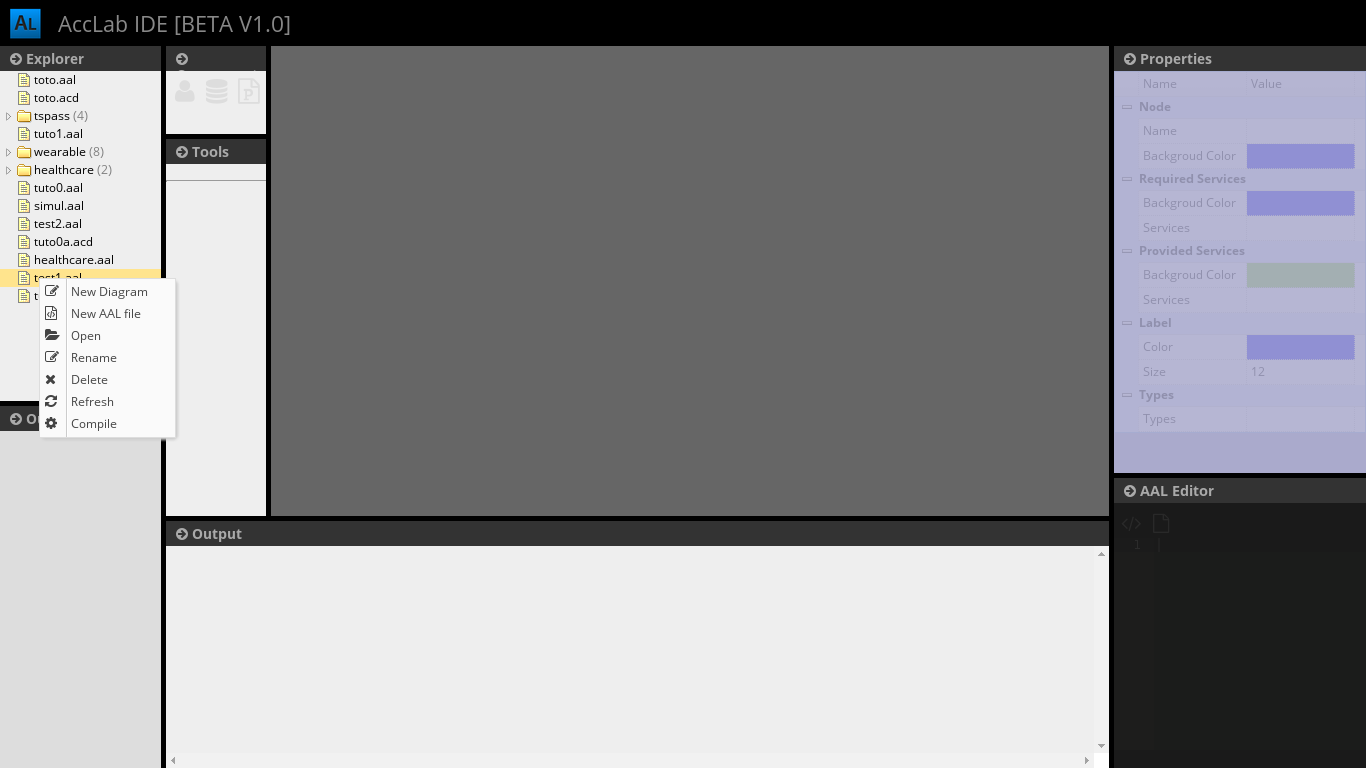
\includegraphics[width=15cm,angle=0]{assets/gui/interface1.png}
      \caption{Creating new diagram}
\end{figure}


\begin{figure}[!ht]
      \center
      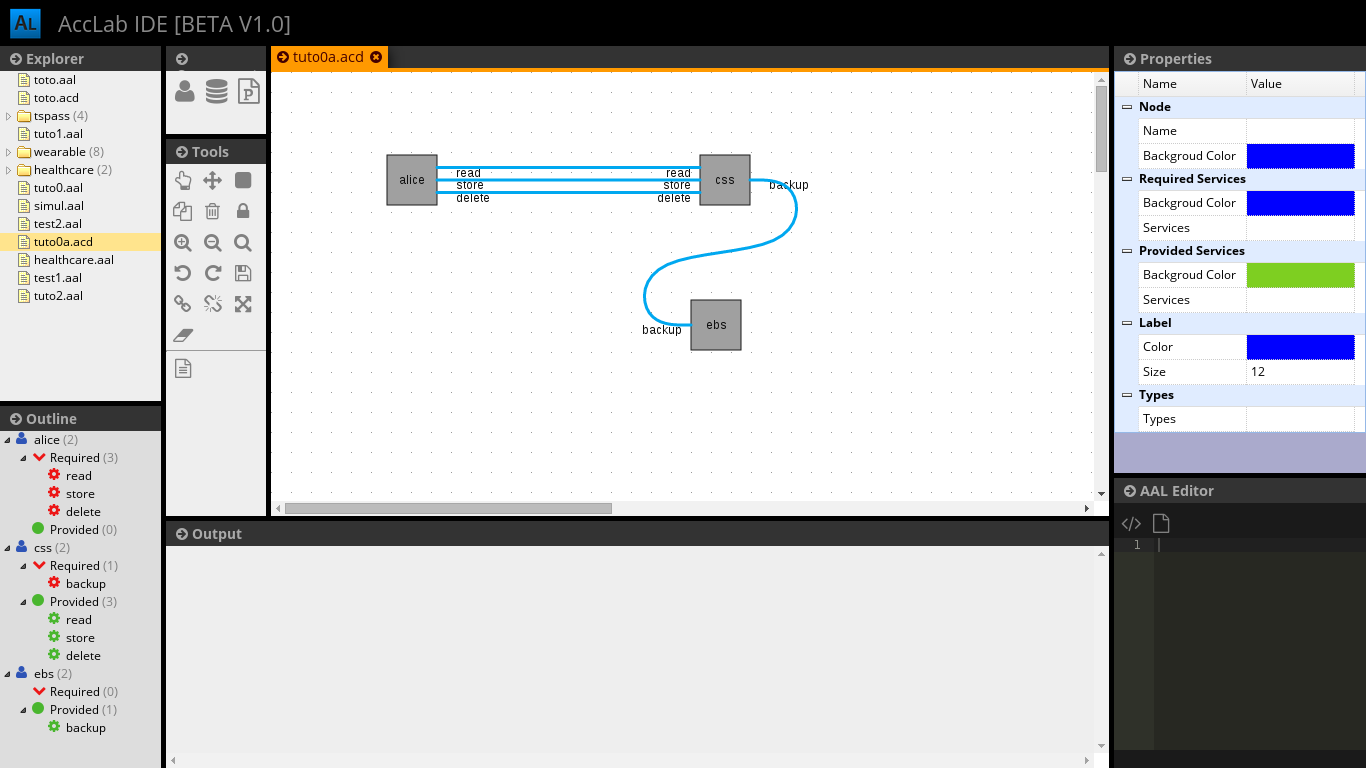
\includegraphics[width=15cm,angle=0]{assets/gui/interface2.png}
      \caption{Editing diagram}
\end{figure}

\begin{figure}[!ht]
      \center
      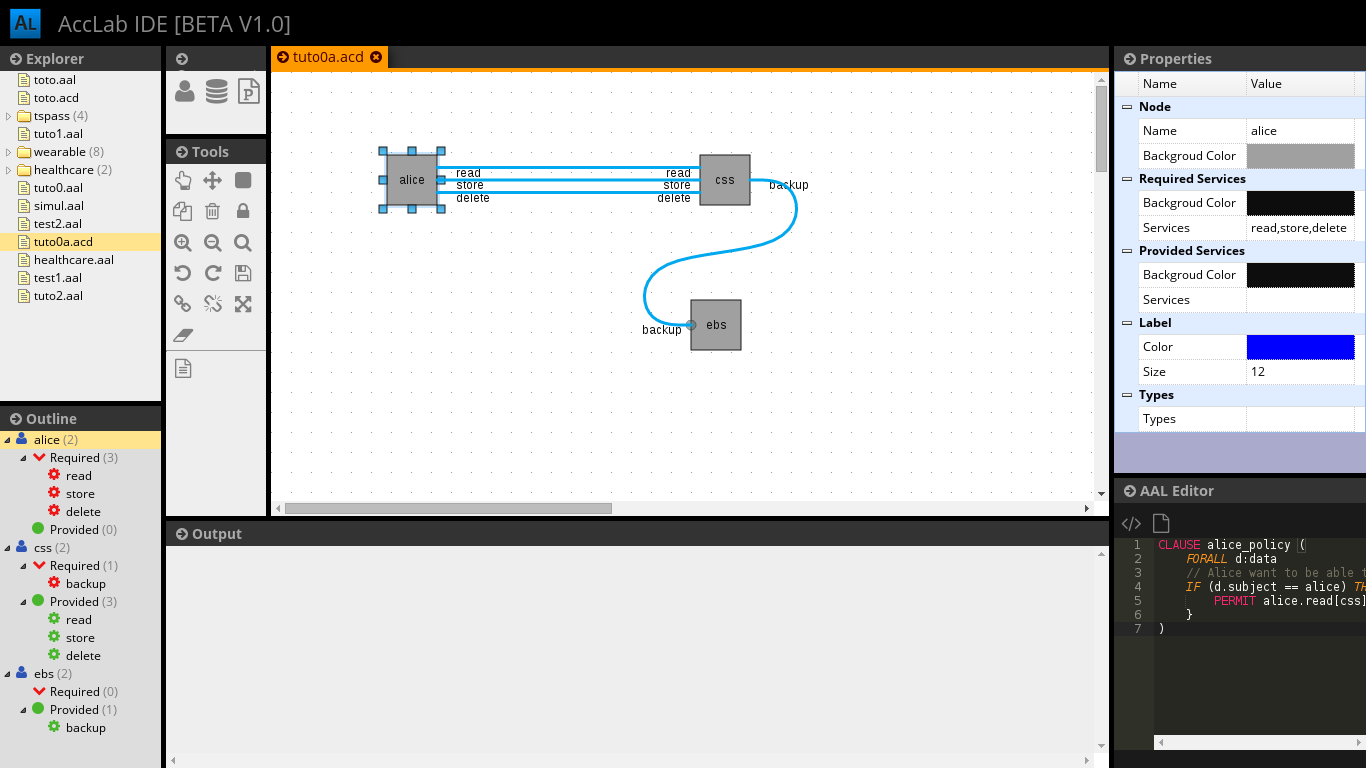
\includegraphics[width=15cm,angle=0]{assets/gui/interface3.png}
      \caption{Adding AAL policies}
\end{figure}

\begin{figure}[!ht]
      \center
      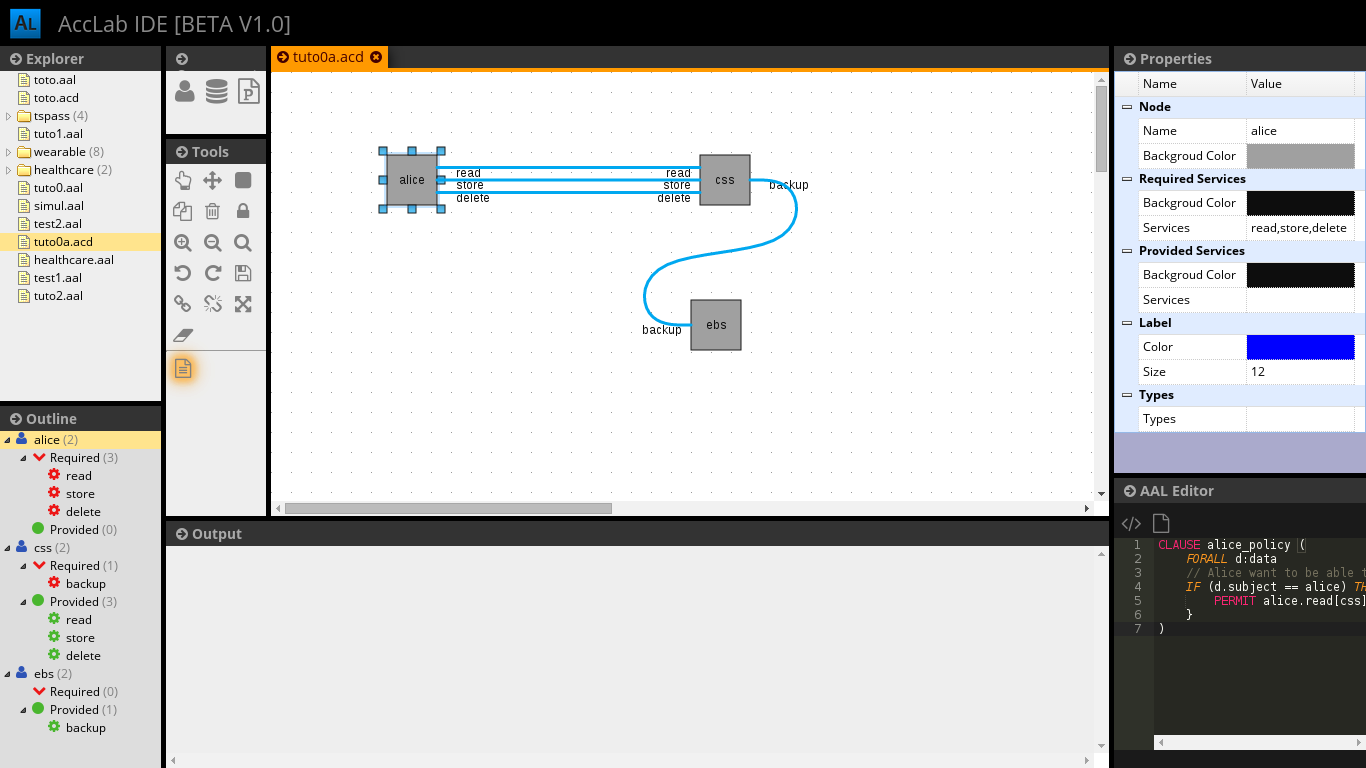
\includegraphics[width=15cm,angle=0]{assets/gui/interface4.png}
      \caption{Generate AAL file}
\end{figure}

\begin{figure}[!ht]
      \center
      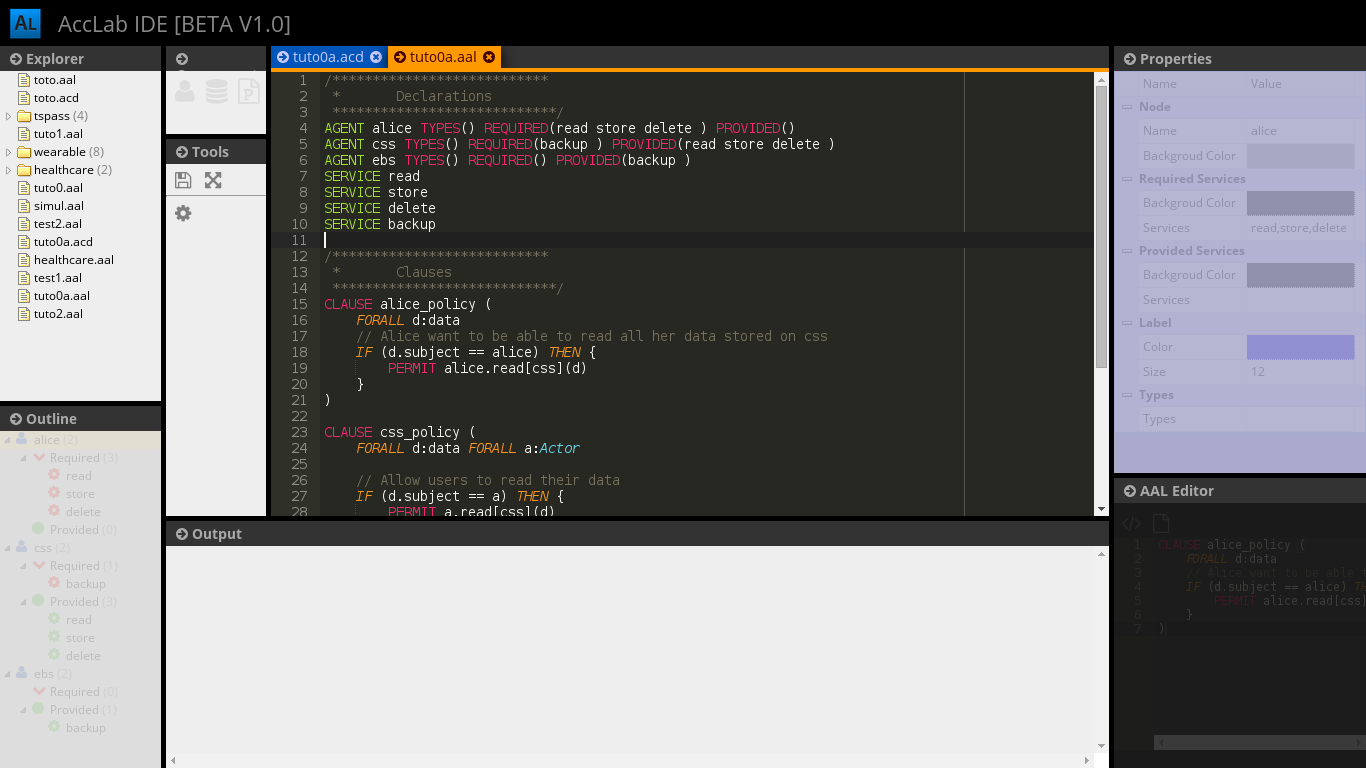
\includegraphics[width=15cm,angle=0]{assets/gui/interface5.png}
      \caption{Generated AAL file}
\end{figure}

\begin{figure}[!ht]
      \center
      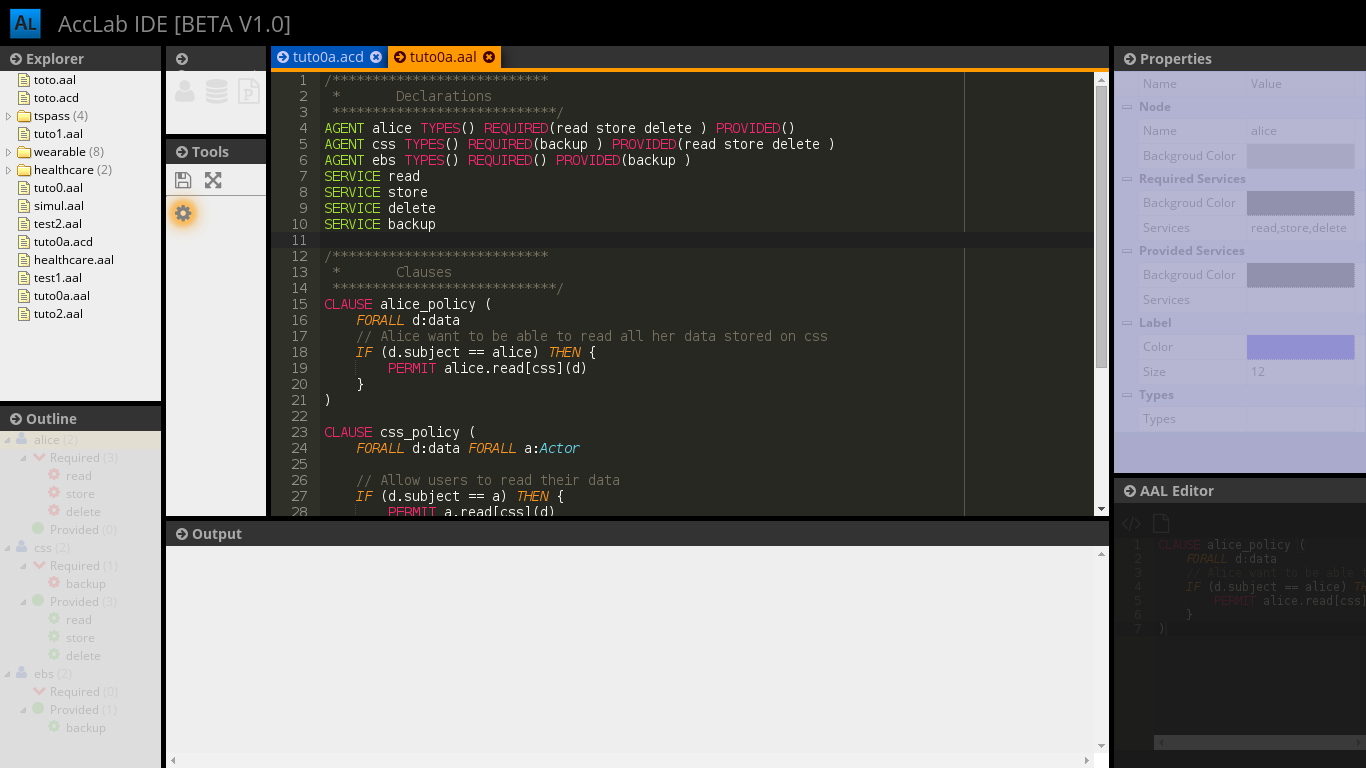
\includegraphics[width=15cm,angle=0]{assets/gui/interface6.png}
      \caption{Compiling AAL file}
\end{figure}

\begin{figure}[!ht]
      \center
      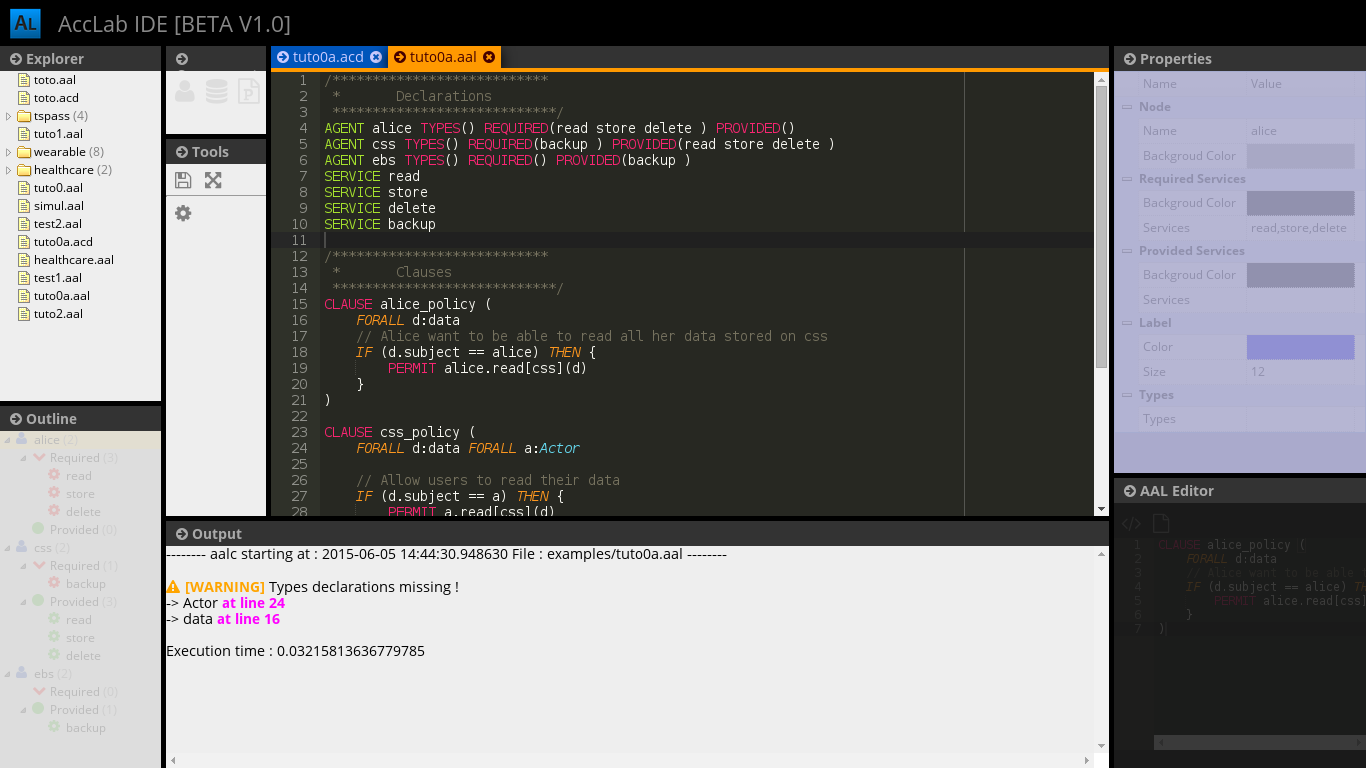
\includegraphics[width=15cm,angle=0]{assets/gui/interface7.png}
      \caption{Result}
\end{figure}

\begin{figure}[!ht]
      \center
      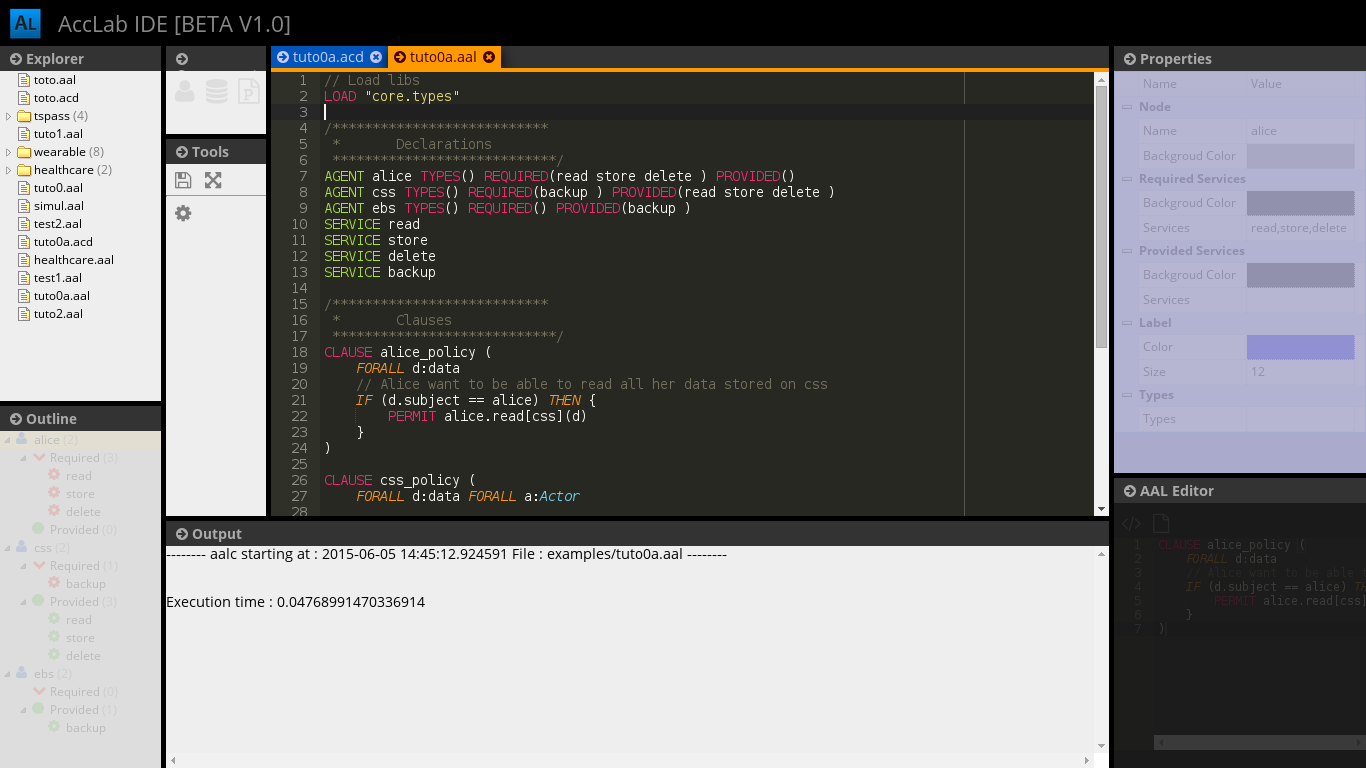
\includegraphics[width=15cm,angle=0]{assets/gui/interface8.png}
      \caption{Load libs}
\end{figure}

\begin{figure}[!ht]
      \center
      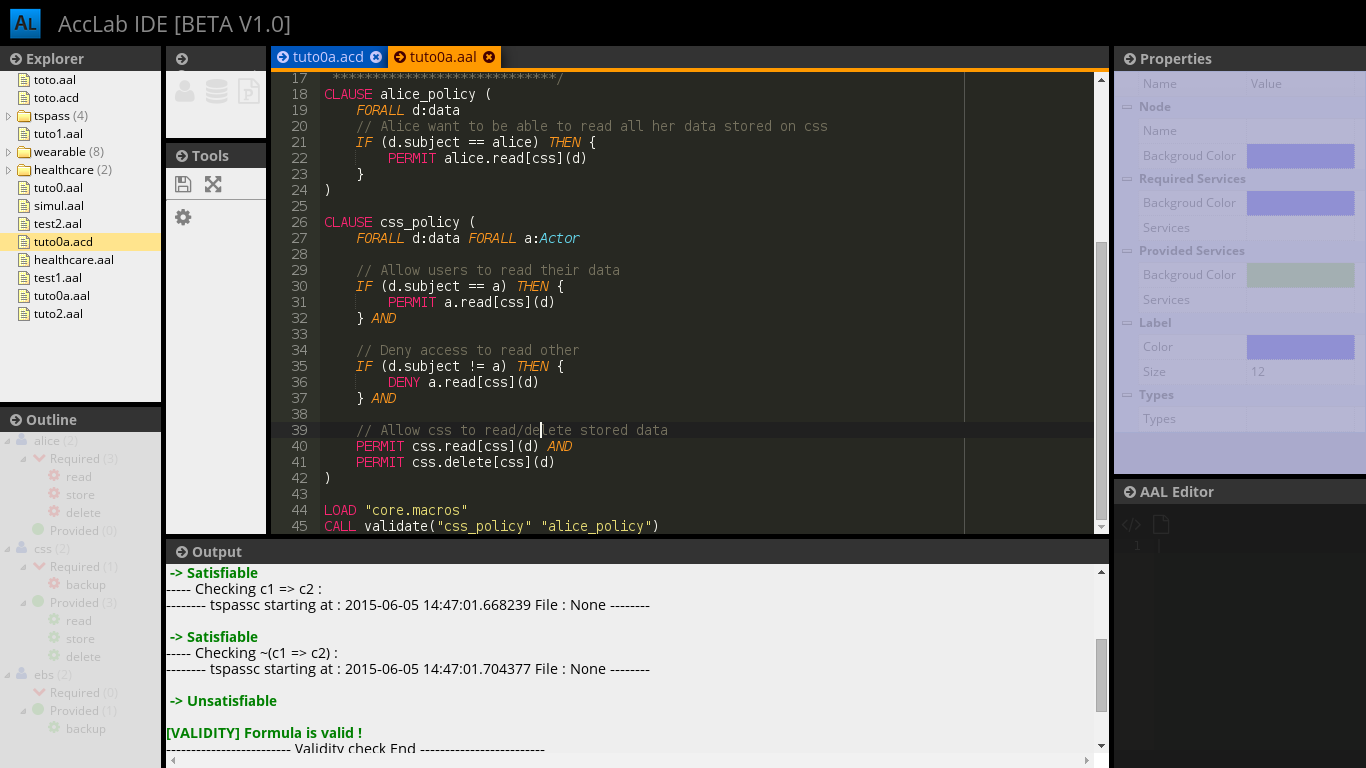
\includegraphics[width=15cm,angle=0]{assets/gui/interface9.png}
      \caption{Validation macro}
\end{figure}
